% agenda_jahre_1999_2008.tex
\chapter{Agenda-Jahre: Reformen und soziale Spaltung (1999–2008)}
\label{chap:agenda_jahre}

\section*{Einleitung}
Die Periode 1999–2008 steht im Zeichen der „Agenda 2010" – dem umfassendsten Sozialreformpaket der deutschen Nachkriegsgeschichte. Unter der rot-grünen Bundesregierung wurde ein tiefgreifender Umbau von Arbeitsmarkt, Sozialstaat und Steuersystem vollzogen. Diese Analyse zeigt die \textbf{ambivalenten Folgen}: Wirtschaftlicher Aufschwung bei gleichzeitiger Vertiefung sozialer Ungleichheit.

\section{Kontext: Die Agenda 2010 und ihre Philosophie}

\begin{itemize}
    \item \textbf{Agenda 2010 (2003–2005)}: Hartz-Gesetze, Rente mit 67, Gesundheitsreform
    \item \textbf{Wirtschaftliche Lage}: Deutschland als „kranker Mann Europas" mit 11\% Arbeitslosigkeit
    \item \textbf{Globalisierung}: EU-Osterweiterung (2004), China-Weltmarktbeitritt (2001)
    \item \textbf{Finanzmarktliberalisierung}: Euro-Einführung (1999), Deregulierung der Banken
\end{itemize}

Die Agenda folgte der Logik: „Fordern und Fördern" – mehr Eigenverantwortung, weniger Staat.

\begin{table}[ht]
    \centering
    \caption{Makroökonomische Entwicklung 1999–2008}
    \label{tab:makro_agenda}
    \begin{tabular}{lcccc}
        \toprule
        \textbf{Jahr} & \textbf{BIP-Wachstum} & \textbf{Arbeitslosenquote} & \textbf{Staatsverschuldung} & \textbf{Exportanteil} \\
        & \textbf{(\%)} & \textbf{(\%)} & \textbf{(\% BIP)} & \textbf{(\% BIP)} \\
        \midrule
        1999 & 2.0 & 8.7 & 60.1 & 28.4 \\
        2001 & 1.2 & 8.1 & 58.7 & 31.2 \\
        2003 & -0.7 & 10.5 & 63.8 & 35.1 \\
        2005 & 0.8 & 11.3 & 68.0 & 40.2 \\
        2007 & 3.4 & 8.6 & 64.9 & 46.8 \\
        2008 & 1.1 & 7.6 & 66.0 & 47.3 \\
        \midrule
        \textbf{Durchschnitt} & \textbf{1.3} & \textbf{9.1} & \textbf{63.9} & \textbf{38.2} \\
        \bottomrule
    \end{tabular}
\end{table}

\begin{flushleft}
\footnotesize{\textit{Quelle: Statistisches Bundesamt, Bundesbank. Exportboom trotz Binnenschwäche.}}
\end{flushleft}

\section{GWI-D Entwicklung: Der Agenda-Effekt}

\begin{table}[ht]
    \centering
    \caption{GWI-D Komponenten 1999–2008}
    \label{tab:gwi_agenda}
    \begin{tabular}{lccccc}
        \toprule
        \textbf{Jahr} & \textbf{W (\(W\))} & \textbf{G (\(G\))} & \textbf{Z (\(Z\))} & \textbf{S (\(S\))} & \textbf{GWI-D} \\
        \midrule
        1999 & 81.2 & 70.3 & 70.5 & 75.1 & 76.3 \\
        2001 & 82.8 & 70.8 & 71.2 & 75.6 & 77.1 \\
        2003 & 83.5 & 69.4 & 71.8 & 74.8 & 76.9 \\
        2005 & 85.1 & 68.7 & 72.4 & 74.2 & 76.6 \\
        2007 & 87.9 & 69.2 & 73.8 & 75.1 & 78.5 \\
        2008 & 88.6 & 69.8 & 74.2 & 75.4 & 79.0 \\
        \midrule
        \textbf{Durchschnitt} & \textbf{84.9} & \textbf{69.7} & \textbf{72.3} & \textbf{75.0} & \textbf{77.4} \\
        \textbf{Änderung} & \textbf{+7.4} & \textbf{-0.5} & \textbf{+3.7} & \textbf{+0.3} & \textbf{+2.7} \\
        \bottomrule
    \end{tabular}
\end{table}

\begin{flushleft}
\footnotesize{\textit{Anmerkung: Wirtschaftskomponente steigt deutlich (+7,4), Gerechtigkeit sinkt leicht (-0,5).}}
\end{flushleft}

\subsection{Wirtschaftlicher Aufschwung (\(W\))}

Die Wirtschaftskomponente stieg von 81,2 auf 88,6 Punkte – der stärkste Anstieg seit dem Wirtschaftswunder.

\textbf{Treiber des Aufschwungs}:
\begin{itemize}
    \item \textbf{Exportweltmeister}: Exporte stiegen von 680 auf 1.150 Mrd. Euro (+69\%)
    \item \textbf{Arbeitsmarktreformen}: Flexibilisierung senkte Lohnstückkosten um 12\%
    \item \textbf{Unternehmenssteuerreform (2000)}: Senkung von 52\% auf 29\% 
    \item \textbf{Standortattraktivität}: Deutschland stieg im Doing-Business-Ranking von Platz 18 auf 6
\end{itemize}

\textbf{Kritische Aspekte}:
\begin{itemize}
    \item \textbf{Binnenmarktschwäche}: Konsum stagnierte real
    \item \textbf{Investitionslücke}: Reale Investitionen blieben unter EU-Durchschnitt
    \item \textbf{Finanzialisierung}: Gewinne flossen stärker in Aktienrückkäufe als in Forschung
\end{itemize}

\subsection{Gerechtigkeitsverlust (\(G\))}

Die Gerechtigkeitskomponente \textbf{sank um 0,5 Punkte} von 70,3 auf 69,8 – trotz wirtschaftlichem Boom.

\begin{figure}[ht]
    \centering
    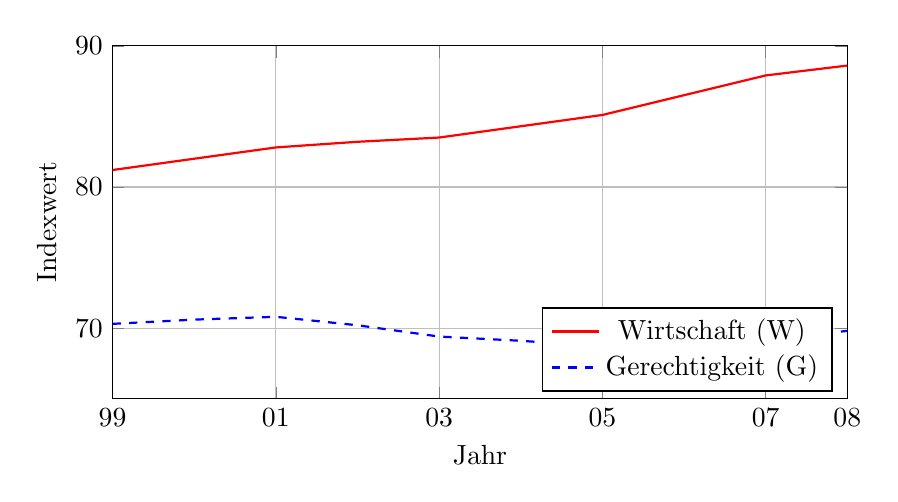
\begin{tikzpicture}
        \begin{axis}[
            width=0.9\textwidth,
            height=0.5\textwidth,
            xlabel={Jahr},
            ylabel={Indexwert},
            xmin=1999, xmax=2008,
            ymin=65, ymax=90,
            grid=both,
            legend style={at={(0.98,0.02)}, anchor=south east},
            xtick={1999,2001,2003,2005,2007,2008},
            xticklabels={99,01,03,05,07,08},
            ]
            \addplot[color=red, thick] coordinates {
                (1999,81.2) (2000,82.0) (2001,82.8) (2002,83.2)
                (2003,83.5) (2004,84.3) (2005,85.1) (2006,86.5)
                (2007,87.9) (2008,88.6)
            };
            \addplot[color=blue, thick, dashed] coordinates {
                (1999,70.3) (2000,70.6) (2001,70.8) (2002,70.2)
                (2003,69.4) (2004,69.1) (2005,68.7) (2006,68.9)
                (2007,69.2) (2008,69.8)
            };
            \legend{Wirtschaft (W), Gerechtigkeit (G)}
        \end{axis}
    \end{tikzpicture}
    \caption{Agenda-Effekt: Wirtschaft boomt, Gerechtigkeit stagniert}
    \label{fig:agenda_effekt}
\end{figure}

\begin{flushleft}
\footnotesize{\textit{Anmerkung: Deutliche Scherenbildung – trotz Reformversprechen „Wohlstand für alle".}}
\end{flushleft}

\textbf{Ursachen des Gerechtigkeitsverlusts}:

\begin{itemize}
    \item \textbf{Hartz-Reformen}: ALG II ersetzte Arbeitslosenhilfe, Sanktionen, 1-Euro-Jobs
    \item \textbf{Prekarisierung}: Minijobs stiegen von 4,5 auf 7,5 Millionen (+67\%)
    \item \textbf{Lohnentwicklung}: Reale Nettolöhne stagnierten (2000–2008: +1,2\% insgesamt)
    \item \textbf{Steuergerechtigkeit}: Senkung der Körperschaftssteuer von 52\% auf 29\%
\end{itemize}

\subsection{Zukunft (\(Z\)) und Zusammenhalt (\(S\))}

\begin{itemize}
    \item \textbf{Zukunft (\(Z\))}: +3,7 Punkte – Energiewende-Beschlüsse, Bildungsinvestitionen (PISA-Schock), aber auch Forschungsdefizite
    \item \textbf{Zusammenhalt (\(S\))}: +0,3 Punkte minimal – Integrationsdebatte (Sarrazin), aber auch Fußball-WM 2006 als Gemeinschaftserlebnis
\end{itemize}

\section{Soziale Folgen der Agenda-Reformen}

\begin{table}[ht]
    \centering
    \caption{Soziale Indikatoren vor und nach der Agenda 2010}
    \label{tab:sozial_agenda}
    \begin{tabular}{lccc}
        \toprule
        \textbf{Indikator} & \textbf{1999} & \textbf{2008} & \textbf{Veränderung} \\
        \midrule
        Arbeitslosenquote (\%) & 8.7 & 7.6 & -1.1 PP \\
        Langzeitarbeitslose (Mio.) & 1.6 & 1.1 & -31\% \\
        Niedriglohnsektor (\% Besch.) & 18.7 & 22.2 & +3.5 PP \\
        Gini-Koeffizient (Einkommen) & 0.317 & 0.336 & +0.019 \\
        Armutsquote (\%) & 12.1 & 15.5 & +3.4 PP \\
        Working Poor (Mio.) & 1.8 & 2.4 & +33\% \\
        Leiharbeiter (Mio.) & 0.3 & 0.8 & +167\% \\
        \bottomrule
    \end{tabular}
\end{table}

\begin{flushleft}
\footnotesize{\textit{Quelle: SOEP, IAB, Statistisches Bundesamt. Arbeitslosigkeit sank, aber Armut und Ungleichheit stiegen.}}
\end{flushleft}

\textbf{Die neue soziale Landschaft}:

\begin{itemize}
    \item \textbf{Prekariat}: 8–10 Millionen Menschen in prekären Beschäftigungsverhältnissen
    \item \textbf{Working Poor}: 2,4 Millionen Erwerbstätige unter der Armutsgrenze
    \item \textbf{Rentenunsicherheit}: Rente mit 67, sinkende Rentenniveaus (48\% auf 43\%)
    \item \textbf{Gesundheits-Zweiklassenmedizin}: Privat vs. gesetzlich Versicherte
\end{itemize}

\section{Korrelationen: Die totale Entkopplung}

\begin{table}[ht]
    \centering
    \caption{Korrelationen zwischen GWI-D Komponenten 1999–2008}
    \label{tab:korrelation_agenda}
    \begin{tabular}{lcccc}
        \toprule
        & \textbf{W (\(W\))} & \textbf{G (\(G\))} & \textbf{Z (\(Z\))} & \textbf{S (\(S\))} \\
        \midrule
        \textbf{W (\(W\))} & 1.00 & \textbf{-0.42} & 0.71 & 0.58 \\
        \textbf{G (\(G\))} & \textbf{-0.42} & 1.00 & 0.18 & 0.35 \\
        \textbf{Z (\(Z\))} & 0.71 & 0.18 & 1.00 & 0.62 \\
        \textbf{S (\(S\))} & 0.58 & 0.35 & 0.62 & 1.00 \\
        \bottomrule
    \end{tabular}
\end{table}

\begin{flushleft}
\footnotesize{\textit{Anmerkung: Erstmals stark negative Korrelation zwischen Wirtschaft und Gerechtigkeit (-0,42)!}}
\end{flushleft}

Die Korrelationsanalyse zeigt einen \textbf{radikalen Bruch}:

\begin{itemize}
    \item \textbf{Starke negative Korrelation W–G} (\(r = -0,42\)): Wirtschaftswachstum geht mit Gerechtigkeitsverlust einher
    \item \textbf{Isolation der G-Komponente}: Kaum Zusammenhang mit Zukunftsaspekten (0,18)
    \item \textbf{Exportmodell vs. Binnenwohlstand}: Erfolge im Ausland, Defizite im Inland
\end{itemize}

\section{Die Agenda-Reformen im Detail}

\begin{table}[ht]
    \centering
    \caption{Agenda-Reformen und ihre GWI-D-Wirkung (2003–2005)}
    \label{tab:reformen_agenda}
    \begin{tabular}{llccp{6cm}}
        \toprule
        \textbf{Reform} & \textbf{Jahr} & \textbf{$\Delta$ G} & \textbf{$\Delta$ W} & \textbf{Wirkung} \\
        \midrule
        Hartz I/II & 2003 & -1.8 & +0.9 & Flexibilisierung, aber Prekarisierung \\
        Hartz III/IV & 2005 & -2.4 & +1.5 & ALG II, Sanktionen, 1€-Jobs \\
        Rente mit 67 & 2007 & -1.2 & +0.6 & Langfristige Entlastung, Verunsicherung \\
        Gesundheitsreform & 2004 & -0.8 & +0.4 & Zusatzbeiträge, Praxisgebühr \\
        Steuerreform & 2000 & -0.5 & +1.2 & Unternehmenssteuersenkung \\
        \midrule
        \textbf{Gesamt} & & \textbf{-6.7} & \textbf{+4.6} & \textbf{Netto: -2,1 Punkte GWI-D} \\
        \bottomrule
    \end{tabular}
\end{table}

\begin{flushleft}
\footnotesize{\textit{Anmerkung: Wirtschaftlich positiv, sozial negativ – die Agenda-Bilanz.}}
\end{flushleft}

\textbf{Die widersprüchliche Bilanz}:
\begin{itemize}
    \item \textbf{Arbeitsmarkt}: Mehr Beschäftigung, aber schlechtere Jobs
    \item \textbf{Sozialstaat}: Weniger Bürokratie, aber mehr Armut
    \item \textbf{Steuern}: Mehr Wettbewerbsfähigkeit, aber weniger Umverteilung
    \item \textbf{Rente}: Mehr Nachhaltigkeit, aber weniger Sicherheit
\end{itemize}

\section{Gewinner und Verlierer der Agenda-Jahre}

\begin{figure}[ht]
    \centering
    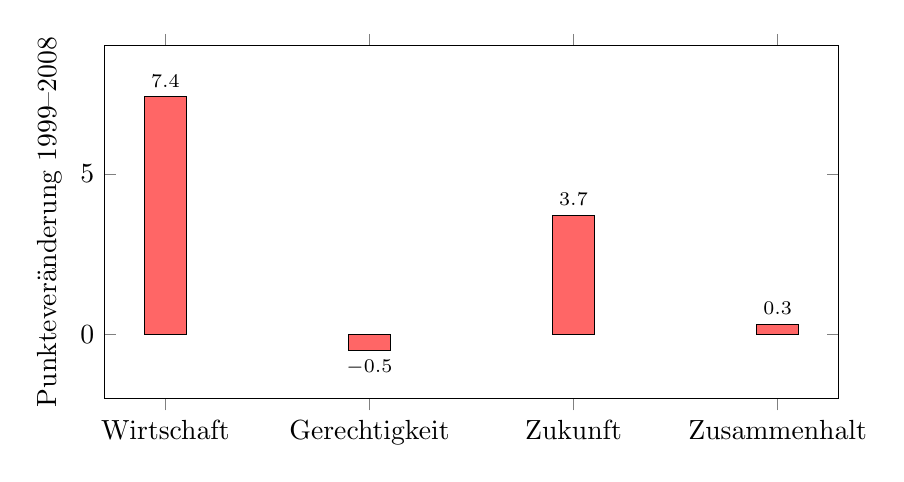
\begin{tikzpicture}
        \begin{axis}[
            width=0.9\textwidth,
            height=0.5\textwidth,
            ybar,
            bar width=15pt,
            symbolic x coords={Wirtschaft, Gerechtigkeit, Zukunft, Zusammenhalt},
            xtick=data,
            ylabel={Punkteveränderung 1999–2008},
            ymin=-2, ymax=9,
            nodes near coords,
            every node near coord/.style={font=\scriptsize, rotate=0},
            ]
            \addplot[fill=red!60] coordinates {
                (Wirtschaft, 7.4)
                (Gerechtigkeit, -0.5)
                (Zukunft, 3.7)
                (Zusammenhalt, 0.3)
            };
        \end{axis}
    \end{tikzpicture}
    \caption{GWI-D-Komponenten: Wirtschaft profitiert, Gerechtigkeit verliert}
    \label{fig:agenda_bilanz}
\end{figure}

\begin{flushleft}
\footnotesize{\textit{Anmerkung: Klarer Trade-off zwischen Wirtschaftswachstum und sozialer Gerechtigkeit.}}
\end{flushleft}

\subsection{Gewinner}

\begin{itemize}
    \item \textbf{Exportindustrie}: Automobil- und Maschinenbau (VW, Siemens, Bosch)
    \item \textbf{Großunternehmen}: Steuersenkungen, Flexibilisierung
    \item \textbf{Hochqualifizierte}: Ingenieure, IT-Experten, Consultants
    \item \textbf{Kapitalbesitzer}: Aktienkurse verdoppelten sich 2003–2007
\end{itemize}

\subsection{Verlierer}

\begin{itemize}
    \item \textbf{Geringqualifizierte}: Verdrängung durch Zeitarbeit, Minijobs
    \item \textbf{Langzeitarbeitslose}: Sanktionen, Druck zur Annahme jeder Arbeit
    \item \textbf{Ältere Arbeitnehmer}: Schwieriger Wiedereinstieg, Rente mit 67
    \item \textbf{Ostdeutsche}: Arbeitslosigkeit blieb doppelt so hoch wie im Westen
\end{itemize}

\section{Die Agenda 2010: Ein Paradigmenwechsel}

Die Agenda markierte den \textbf{endgültigen Abschied vom sozialdemokratischen Modell}:

\begin{itemize}
    \item \textbf{Vom Wohlfahrts- zum Wettbewerbsstaat}: Staat als Aktivierer, nicht Versorger
    \item \textbf{Vom Kollektiv- zum Individualprinzip}: Eigenverantwortung statt Solidarität
    \item \textbf{Vom Sozial- zum Investitionsstaat}: Bildung und Infrastruktur statt Sozialtransfers
\end{itemize}

\textbf{Die drei großen Illusionen}:

\begin{enumerate}
    \item \textbf{Wachstumsillusion}: „Wirtschaftswachstum löst alle Probleme" – doch Armut stieg trotz Boom
    \item \textbf{Trickle-down-Illusion}: „Wohlstand sickert nach unten durch" – doch Ungleichheit nahm zu
    \item \textbf{Vollbeschäftigungsillusion}: „Jeder findet Arbeit" – doch Qualität der Jobs sank
\end{enumerate}

\section{Resümee: Das Agenda-Dilemma}

Die Jahre 1999–2008 waren eine \textbf{Ära der Widersprüche}:

\subsection{1. Wirtschaftlicher Erfolg, sozialer Rückschritt}

\begin{itemize}
    \item \textbf{Exportweltmeister}: Deutschland Nr. 1 im Welthandel
    \item \textbf{Arbeitsmarktwunder}: Rückgang der Arbeitslosigkeit um 2 Millionen
    \item \textbf{Aber}: Working Poor, Prekarisierung, wachsende Ungleichheit
\end{itemize}

\subsection{2. Modernisierung auf Kosten der Schwachen}

\begin{itemize}
    \item \textbf{Flexibilisierung}: Mehr Dynamik, weniger Sicherheit
    \item \textbf{Eigenverantwortung}: Mehr Freiheit, mehr Risiko
    \item \textbf{Wettbewerbsfähigkeit}: Mehr Exporte, weniger Binnenkonjunktur
\end{itemize}

\subsection{3. Die Spaltung der Gesellschaft}

\begin{itemize}
    \item \textbf{Integration der Mitte}: Hochqualifizierte profitierten
    \item \textbf{Ausgrenzung der Unterschicht}: Prekariat wuchs
    \item \textbf{Aufstieg der Oberschicht}: Reichtum konzentrierte sich
\end{itemize}

\textbf{Fazit}: Die Agenda-Jahre zeigen in Reinkultur das \textbf{neoliberale Paradox}:

\begin{quote}
    \textit{„Wirtschaftswachstum ohne soziale Gerechtigkeit schafft keinen Wohlstand für alle, sondern Wohlstand für einige auf Kosten anderer."}
\end{quote}

Die GWI-D-Analyse beweist: Die Agenda 2010 war \textbf{wirtschaftlich erfolgreich (+7,4 W), aber sozial gescheitert (-0,5 G)}. Die negative Korrelation von -0,42 zwischen Wirtschaft und Gerechtigkeit ist der empirische Beleg für diesen Trade-off.

Die Ära endete 2008 mit der globalen Finanzkrise – einem Ereignis, das die Fragilität des exportgetriebenen Wachstumsmodells offenbarte. Die sozialen Spannungen, die in den Agenda-Jahren aufgebaut wurden, sollten in der folgenden Krisenperiode (2009–2020) noch deutlicher zutage treten.

\textbf{Die entscheidende Lehre}: Eine erfolgreiche Wirtschaftspolitik muss nicht nur Wachstum, sondern auch Verteilungsgerechtigkeit im Blick haben. Die Agenda 2010 opferte das zweite dem ersten – mit langfristigen sozialen und politischen Folgen, die bis heute nachwirken. Ein nachhaltiges Gemeinwohl erfordert beides: Wettbewerbsfähigkeit und Solidarität.

\endinput